\documentclass[a4paper,12pt]{article}

\usepackage{graphicx}
\usepackage{url}
\usepackage{xcolor}

\setlength{\parskip}{\baselineskip}%
\setlength{\parindent}{0pt}%

\begin{document}

\title{Large Scale Sentiment Analysis of Tweets }%replace with the appropriate homework number
\author{
	James Tan Juan Whei\\
	Concordia University
}  
\maketitle

\begin{abstract}
Abstract, here is what an abstract is compared to an intro

https://www.discoverphds.com/blog/abstract-vs-introduction
\end{abstract}

\section{Introduction}

An idea of what the project is about and its possible use cases?

\section{Tools and Technologies}
An introduction to the tools that were used and why they were chosen for this project

\subsection{GCS}
Some description about GCS

\subsection{BigQuery}
Some description about BigQuery

\subsection{Dataproc and Spark}
\label{sec:spark}
Some description about Dataproc and Spark. Mention cluster configuration, number of instances, type of instances, etc. Refer readers to our scripts for specifics.

\section{Dataset}
\label{sec:dataset}
We relied heavily on the snscrape library\footnote{Scraper for social networking services (SNS): https://github.com/JustAnotherArchivist/snscrape} to scrape tweets. We filtered for tweets that were in the English language only. Approximately 1000000 tweets were scraped for each day between 2022-05-01 and 2022-07-12. The tweets were then saved in Google Cloud Storage.

\section{Processing of Data}

As mentioned in Section \ref{sec:spark}, we define the processing of the data as a Spark job. The steps involved in the job are illustrated in Figure \ref{fig:data-processing-pipeline} and will be further elaborated on in the subsequent sections. Our processing pipeline relies heavily on the Spark NLP library\footnote{Spark NLP: State of the Art Natural Language Processing: https://nlp.johnsnowlabs.com}.

\begin{figure}[h]
\centering
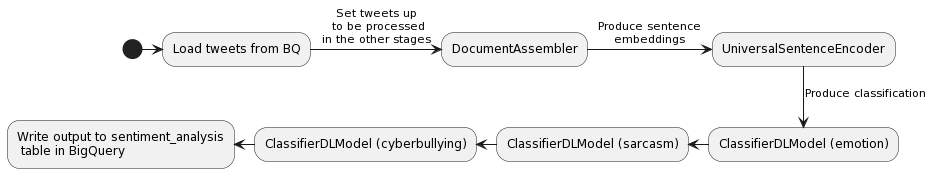
\includegraphics[width=\textwidth]{data-processing.png}
\caption{The processing pipeline}
\label{fig:data-processing-pipeline}
\end{figure}

\subsection{Data Ingestion}
In order to use data stored in BigQuery as an input to our Spark job, we used the Spark BigQuery connector\footnote{Use the BigQuery connector with Spark: https://cloud.google.com/dataproc/docs/tutorials/bigquery-connector-spark-example}. The Spark script reads from a table that contains all the tweets that were procured as described in Section \ref{sec:dataset}. 

Each run of the Spark job would typically be executed on 4-5 days' worth of tweets as we discovered that the Spark jobs had a tendency of failing when working with larger amounts of data. This was true even when the CPU and memory utilization of the worker nodes were relatively healthy and thus should be further investigated.

\subsection{Document Assembler}
The first step of the pipeline is the \texttt{DocumentAssembler}\footnote{https://nlp.johnsnowlabs.com/api/com/johnsnowlabs/nlp/DocumentAssembler}. This prepares the data into a format that is processable by Spark NLP and is essentially the entry point for every Spark NLP pipeline.

\subsection{Generation of Sentence Embeddings}
\label{sec:sentence-embeddings}
We generate sentence embeddings by leveraging a Universal Sentence Encoder\footnote{https://www.tensorflow.org/hub/tutorials/semantic\_similarity\_with\_tf\_hub\_universal\_encoder?hl=en} made available by Tensorflow. The output of this stage is a 512-dimensional vector that semantically captures the meaning of each tweet. This is the basis upon which the downstream classification algorithms build on.

\subsection{Sentiment Classification}
To actually use the embeddings described in the previous section, we utilise ClassifierDLModels\footnote{https://nlp.johnsnowlabs.com/api/com/johnsnowlabs/nlp/annotators/classifier/dl/ClassifierDLModel.html} to classify the tweets. Each ClassifierDLModels essentially assigns a label to each tweet. To identify the emotion, presence of cyberbullying and presence of racism in each tweet, we use the \texttt{classifierdl\_use\_emotion}, \texttt{classifierdl\_use\_cyberbullying} and \texttt{classifierdl\_use\_sarcasm} pretrained models respectively ({\color{red}TODO: Better way of phrasing this?}). 

The emotion classifier produces the values \texttt{sadness}, \texttt{joy}, \texttt{love}, \texttt{anger}, \texttt{fear} and \texttt{surprise}. The cyberbullying classifier produces the values \texttt{neutral}, \texttt{racism} and \texttt{sexism}. The sarcasm classifier produces the values \texttt{sarcasm} and \texttt{normal}. 

\subsection{Storing of Output}
The output is then stored in a separate table in BigQuery. Note that the BigQuery Spark connector is once again used here, thus allowing the output of a Spark job to be appended directly to a BigQuery table.

\section{Results}
TODO: Some visualizations and the insights we obtained

\section{Future Work}
An idea that we originally had was to run an unsupervised clustering algorithm on the sentence embeddings produced in Section \ref{sec:sentence-embeddings}. The clustering algorithm that we had in mind was DBScan\cite{Ester96adensity-based}, with the objective of clustering tweets with similar topics. Unfortunately, we were not able to find a satisfactorily efficient implementation of the algorithm to employ with Spark. Due to the size of our dataset and the high number of dimensions of the embeddings, an efficient implementation was crucial to the success of this idea. Given that we had limited resources, we were forced to abandon this idea, however, it should be revisited in the future by implementing our own version of the DBScan algorithm.

\section{Code}
The code to reproduce our project may be found in our Github repository.\footnote{Github repository of the project: https://github.com/jamestjw/tweet\_analysis\_comp6231} 

\section{Conclusion}
We worked hard and achieved very little.

\nocite{*}

\bibliographystyle{abbrv}
\bibliography{main.bib}

\end{document}  
